\chapter{Diseño electrónico de un canal de lectura}\label{cap:ro_sch}

\paragraph{}
El canal de lectura es el circuito que lee la información almacenada en los píxeles
tras el tiempo de exposición.
En la arquitectura más habitual, y la que vamos a tratar en este estudio, los
píxeles se leen por columnas, entendiéndose que el chip tiene una dirección
\textit{vertical} y otra \textit{horizontal}. Siguiendo ese criterio, el canal de lectura se
sitúa debajo del array de píxeles de forma que cada columna del canal quede alineada
con cada columna del canal.

\paragraph{}
Idealmente podríamos un canal por columna, y meter en ese espacio todo el circuito
para la columna. Pero, en algunos casos, debido al pequeño tamaño de los píxeles
--- suelen tener unos 5, 8, 10$\mum$... --- resulta complicado o incluso imposible diseñar el
layout de dicha circuitería en ese reducido espacio horizontal. De ahora en adelante
usaremos la palabra inglesa \textit{``pitch''} para referirnos al espaciado con el
que se repite una estructura periódica como el canal de lectura o el array.

\paragraph{}
Por esta razón, es una práctica común usar el \textit{pitch} de varios píxeles, por
ejemplo 2 ó 4, y así tener más espacio para diseñar el layout del circuito. Por contra,
debemos apilar estos 2 ó 4 canales en filas, lo que veremos que nos trae algunos
problemas a la hora de diseñar el layout.

\paragraph{}
De ahora en adelante nos centraremos en el caso de un sensor cuyos píxeles tengan
un área de $5\mum \times 5\mum$, y en el que se apilan 2 canales para leer 2
columnas de píxeles. Por tanto, el ancho de un canal será de $10\mum$, encajando
exáctamente en la anchura de 2 columnas de píxeles.

\section{Estructura general}\label{cap:ro_sch_estructura}

\paragraph{}
El canal de lectura es un circuito analógico que va a convertir el voltaje
dado por el pixel tras haber sido expuesto a la luz durante un tiempo y
convertirlo en un valor analógico bien definido entre unos límites que van a
significar \textit{blanco} y \textit{negro}, con una resolución definida.

\paragraph{}
Por tanto, el canal de lectura es principalmente un ADC (en inglés, \textbf{A}nalog
to \textbf{D}igital \textbf{C}onverter, o convertidor analógico-digital).
Una arquitectura usada habitualmente es el convertidor de rampa.
Éste, para la conversión usa un generador de una rampa de voltaje que se usa para
comparar contra el valor dado por el píxel. Ćuando ambos valores coinciden,
la salida del comparador cambia de estado mediante un flanco de subida o bajada.
De ésta forma la conversión de un valor de tensión se traduce en la detección temporal
de un flanco.

\paragraph{}
De manera simultánea a la rampa analógica se lanza una rampa digital que va contando
valores desde 0 hasta un número que viene determinado por la resolución, y que va a
evolucionar a la misma velocidad que la analógica. Posteriormente, un circuito digital
detectará el flanco y parará el reloj de la cuenta digital, obteniéndose de esta forma
un valor digital para el valor analógico leído.

\paragraph{}
Entre las ventajas de usar un convertidor de rampa frente a otras muchas posibilidades
que existen en la literatura para convertir valores analógicos a digitales, podemos
destacar las siguientes:

\begin{enumerate}
	\item Se trata de un circuito muy simple, que puede reducirse a un comparador
	creado con un OTA simple de 5 transistores, más un par de condensadores y
	algunas llaves. Cualquier otra arquitectura (convertidor SAR, sigma-delta...)
	implican muchos más transistores y posiblemente más consumo.
	\item Se puede obtener una buena linealidad si se diseña una buena rampa
	y se hace operar al comparador en un punto de operación similar en todos los casos,
	consiguiendo ecualizar los tiempos de transición del mismo.
	\item Es fácilmente repetible en todas las columnas, ya que podemos separar
	la generación de la rampa de los comparadores.
\end{enumerate}

\section{Operación de lectura}\label{cap:ro_sch_operacion}

\paragraph{}
Para abordar el diseño de un canal de lectura debemos entender como se realiza la
operación de lectura de los píxeles.

\paragraph{}
En la figura \ref{fig:pixel} podemos ver el esquemático de el pixel 5T
que vamos a usar para este estudio. El fotodiodo (PD), es el elemento que más
área ocupa del pixel, ya que es el area que recibe los fotones.

\begin{figure}[h]
	\centering
	\begin{subfigure}{0.6\textwidth}
		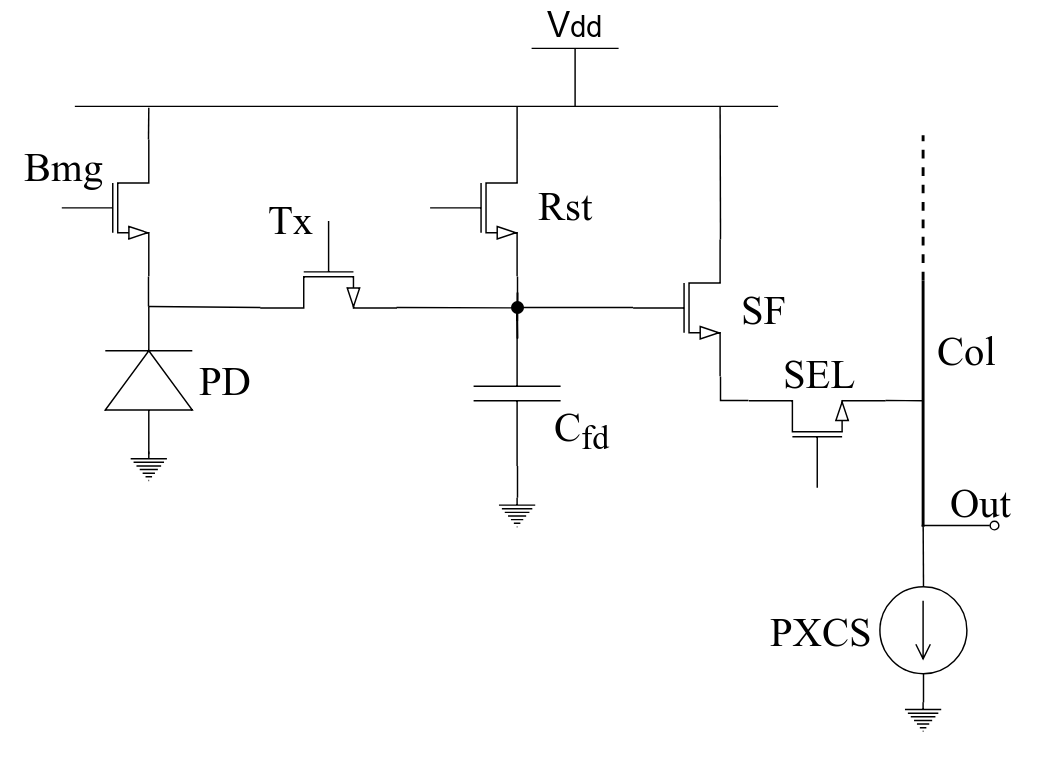
\includegraphics[width=\textwidth]{img/pixel_5T.png}
		\caption{}
		\label{fig:pixel}
	\end{subfigure}

	 %add desired spacing between images, e. g. ~, \quad, \qquad, \hfill etc.
	%(or a blank line to force the subfigure onto a new line)
	\begin{subfigure}{\textwidth}
		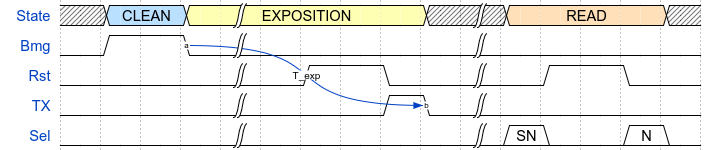
\includegraphics[width=\textwidth]{img/pixel_wave.png}
		\caption{}
		\label{fig:pixel_op}
	\end{subfigure}
	\caption{Esquemático y modo operación de un pixel 5T habitual}
\end{figure}

\paragraph{}
Mirando el modo de operación (\ref{fig:pixel_op}) vemos que antes de la exposición se hace un vaciado del
fotodiodo mediante el transistor de BMG, que coloca una tensión alta en el fotodiodo.
Durante la exposición, los electrones fotogenerados van bajando la tensión de este
nodo. Para terminar la exposición, se hace una transferencia de esta carga hacia
el condensador $C_{fd}$ (\textit{Floating Diffusion}), no sin antes dar un pulso
en el transistor de RST (Reset), para vaciar la posible carga que tuviera este condensador.

\paragraph{}
En este punto tenemos la carga con la información de la luz captada por el pixel,
almacenada en el condensador $C_{fd}$, a la espera de que queramos leer este valor
mediante la activación del transistor SEL (Selección). Normalmente, para compensar
errores debidos a asimetrias en los píxeles, se hace una operación de CDS, siglas de
``\textit{Correlated Double Sampling}''. Esto es, medir la señal bruta que tenemos
en la ``floating diffusion'', e inmediatamente después, limpiar este condensador con
un pulso de Reset y volver a leer. De esta forma, simbolizando con S, señal y N,
ruido (\textit{noise}), si restamos ambas formas de onda, podemos obtener:

\begin{equation}
	\label{eq:CDS_operation}
	S = SN - N
\end{equation}

\paragraph{}
Podemos hacer esto debido a que ambas medidas  están correlacionadas porque se
hacen con muy poco tiempo de diferencia y entonces los ruidos son aproximadamente
iguales.

\paragraph{}
Habitualmente existen dos formas de exponer el array: ``\textit{global shutter}'',
obturación global, y ``\textit{rolling shutter}'', obturación consecutiva. En la
primera, todas las filas del array se exponen simultáneamente y luego, fila por fila
se van leyendo los valores almacenados en las ``\textit{floating diffusions}''. En
el segundo caso, la exposición se hace secuencialmente, fila por fila, antes de cada
lectura.

\section{Fuente de corriente}\label{cap:ro_sch_pxcs}
\paragraph{}
La fuente de corriente, normalmente abreviada como PXCS (del inglés,
\textbf{P}i\textbf{x}el \textbf{C}urrent \textbf{S}ource),
es el primer bloque que se sitúa en
en el canal de lectura y es común a todas las filas de píxeles. Básicamente
es un transistor polarizado en saturación, de modo que drena una corriente
constante que copia de otro transistor con el que forma un espejo de corrientes.
Podemos ver un esquemático del circuito habitual en la figura \ref{fig:pxcs_sch}.

\paragraph{}
Normalmente, la corriente es configurable, para permitir tiempos de lectura menores
incrementando su  valor, o por el contrario, disminuir el consumo si no necesitamos tanta
velocidad.

\begin{figure}[h]
	\centering
	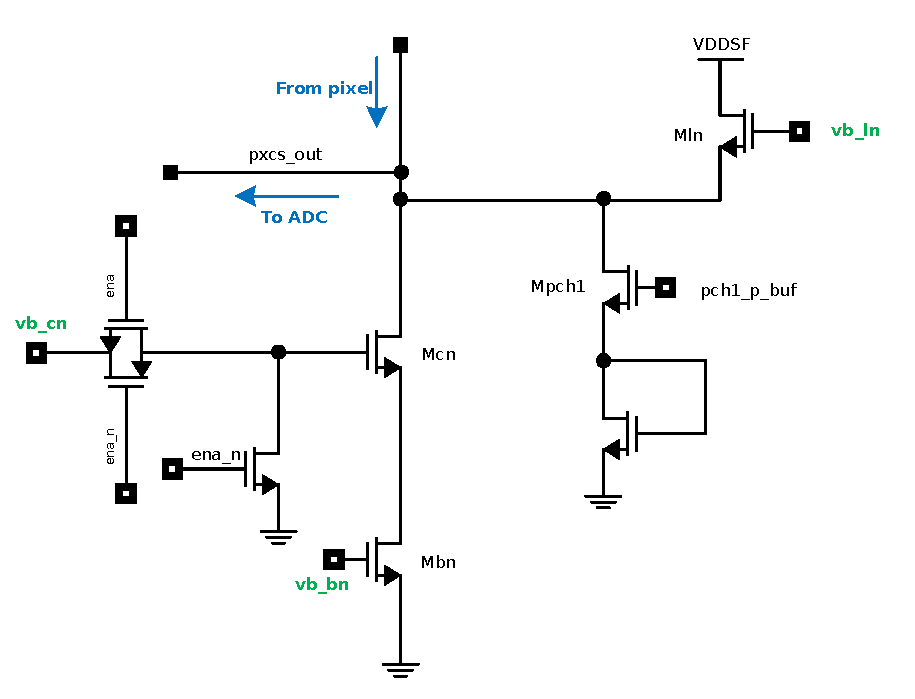
\includegraphics[width=0.8\textwidth]{svg/pxcs_sch.pdf}
	\caption{Esquemático de la fuente de corriente del pixel}
	\label{fig:pxcs_sch}
\end{figure}

\paragraph{}
La rama que va a tierra desde el nodo de salida del bloque se usa para la pre-carga.
La llamada pre-carga es un sistema que se usa habitualmente para hacer que el
establecimiento de la señal cargada por la fuente de corriente se haga más rápido
y en las mimas condiciones siempre. Lo que se hace es dar un pulso de pre-carga
(\textit{pch}) un poco antes de activar el \textit{sel}. Ésta rama hace bajar la
tensión de salida del píxel a un valor cercano a cero para empezar a evolucionar
desde ahí al valor de la \textit{floating diffusion} menos el $V_{gs}$ del seguidor
por fuente (SF) del píxel.
%WARNING
%Continuar aquí y explicar mejor precarga y limitador


\section{Convertidor de rampa}\label{cap:ro_sch_conv}

\paragraph{}
Como ya hemos comentado, la conversión del valor analógico del pixel, a un número
digital se realiza mediante un convertidor de rampa. Para conseguir esto,
en cada canal de lectura se implementa un sencillo ADC comparador y unos condensadores
dónde almacenar temporalmente las señales.

\paragraph{}
La señal de la rampa analógica se va a distribuir horizontalmente entre todas las
columnas del canal de lectura, y está generada por un bloque externo al RO, situado
a uno de los lados del mismo, con lo que evitamos incluirlo en area del canal.


\section{ADC}\label{cap:ro_sch_adc}

\paragraph{}
El ADC es el bloque que muestrea y compara la señal analógica del píxel con la de la
rampa analógica. El esquemático del circuito se muestra en la figura \ref{fig:adc_sch}.
La operación del ADC se realiza en 2 fases, lectura (\textit{read}) y comparación
(\textit{comp}), y se puede seguir mediante las formas de onda mostradas en \ref{fig:adc_wave}.

\begin{figure}[h]
	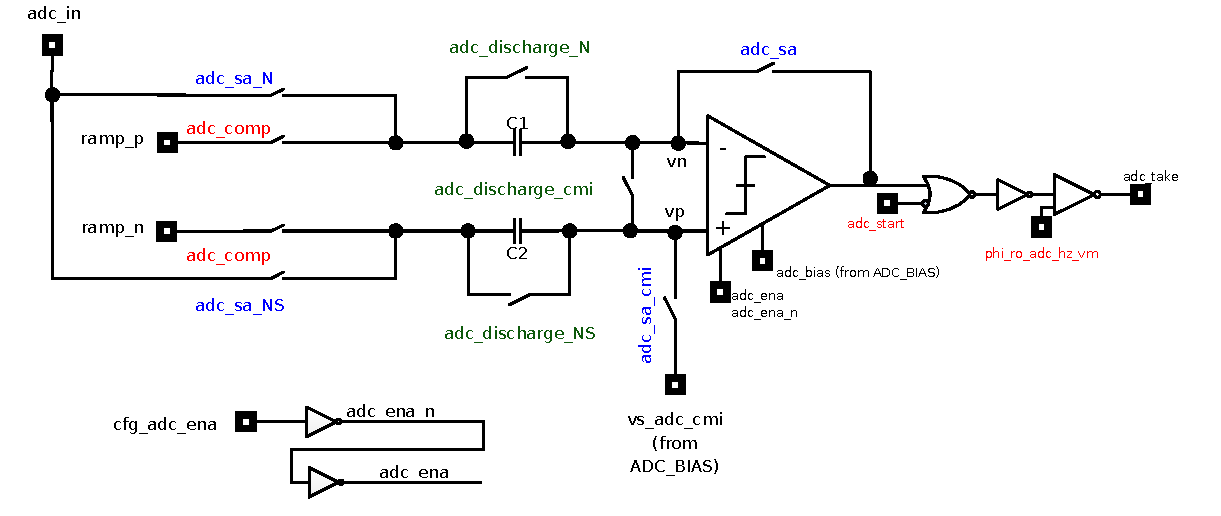
\includegraphics[width=\textwidth]{svg/adc_sch.pdf}
	\caption{Esquemático del ADC}
	\label{fig:adc_sch}
\end{figure}

\begin{figure}[h]
	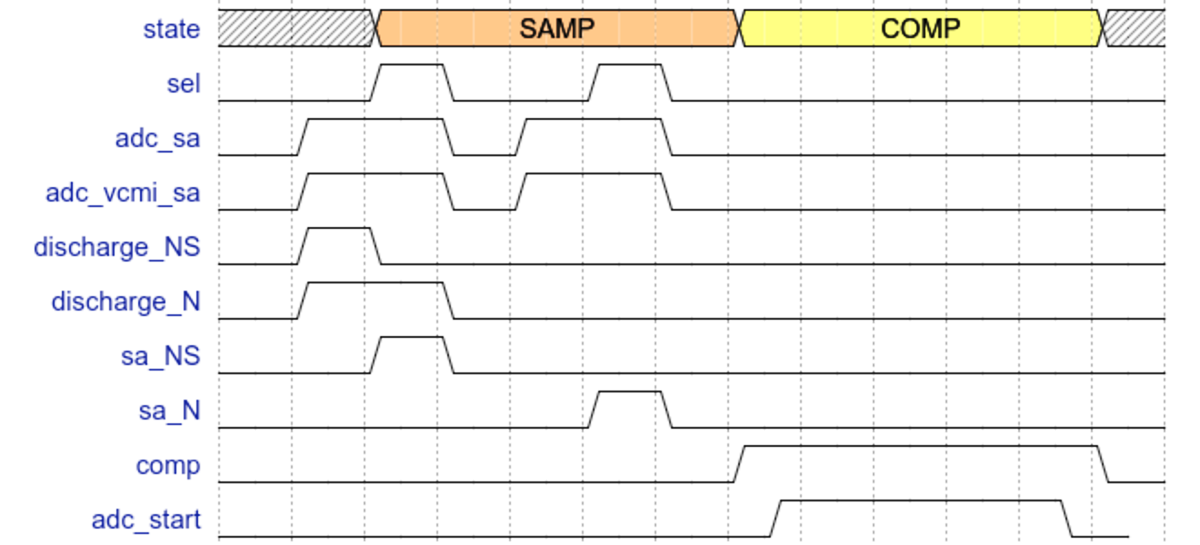
\includegraphics[width=\textwidth]{img/adc_wave.png}
	\caption{Señales de onda del comparador de rampa}
	\label{fig:adc_wave}
\end{figure}

\paragraph{}
Durante la primera de ellas, el comparador está operando en lazo cerrado, por lo
los nodos de entrada $vp$ y $vn$ se establecen a la tensión de modo
común, $vs\_adc\_cmi$. Al final del periodo de muestreo, las señales
``señal + ruido'' (NS) y ``ruido'' (N), quedan almacenadas en los condensadores $C_2$
y $C_1$, respectivamente.

\paragraph{}
En la segunda fase, el comparador se establece en lazo abierto, por lo que la carga
almacenada en los condensadores se mantiene. En ese momento se conecta la
rampa diferencial ($ramp_P$ y $ramp_N$), y aplicando la conservación de carga en los
nudos $vp$ y $vn$, se puede deducir que el voltage será:

\begin{align}
	v_n &= \dfrac{v_{cmi} + v_{off}}{1+\frac{1}{A_0}} + \alpha_1 (v_{ramp_p}-v_{pixN})\\
	v_p &= v_{cmi} + \alpha_2 (v_{ramp_n}-v_{pixNS})
\end{align}
, dónde los coeficientes $\alpha_1$ y $\alpha_2$ son:

\begin{equation}
	\alpha_1 = \dfrac{C_1}{C_1+C_p},~
	\alpha_2 = \dfrac{C_2}{C_2+C_p}
\end{equation}

\paragraph{}
Asumiendo un comparador ideal, el voltage diferencial a la entrada de este, se
puede expresar como:

\begin{equation}
	\Delta V= v_p - v_n = (v_{pixNS}-v_{pixNS}) - (v_{ramp_p}-v_{ramp_n})
\end{equation}

, dónde la diferencia $(v_{pixNS}-v_{pixNS})$ es siempre positiva y se relaciona
con la información almacenada en el píxel, y la señal $(v_{ramp_p}-v_{ramp_n})$ es
linealmente creciente. Por tanto, la salida del comparador debe ser inicialmente
un valor alto y cambiar a valor bajo en el instante en que ambas señales sea crucen.
Por lo que la información en el píxel puede codificarse con el tiempo registrado
por un contador digital, siendo mayor el número digital a mayor la luz recibida
por el pixel leído.

\paragraph{}
La salida del comparador se hace pasar por una puerta NOR para evitar que pueda
registrarse una transición sin estar activa la señal de $adc\_start$

\subsection{OTA}\label{cap:ro_sch_ota}

\paragraph{}
El OTA (\textit{Operational Transconductance Amplifier}) es el bloque que actúa
cómo comparador y tiene la estructura de un amplificador diferencial simple, que
se muestra en el esquemático de la figura \ref{fig:ota_sch}.

\begin{figure}[h]
	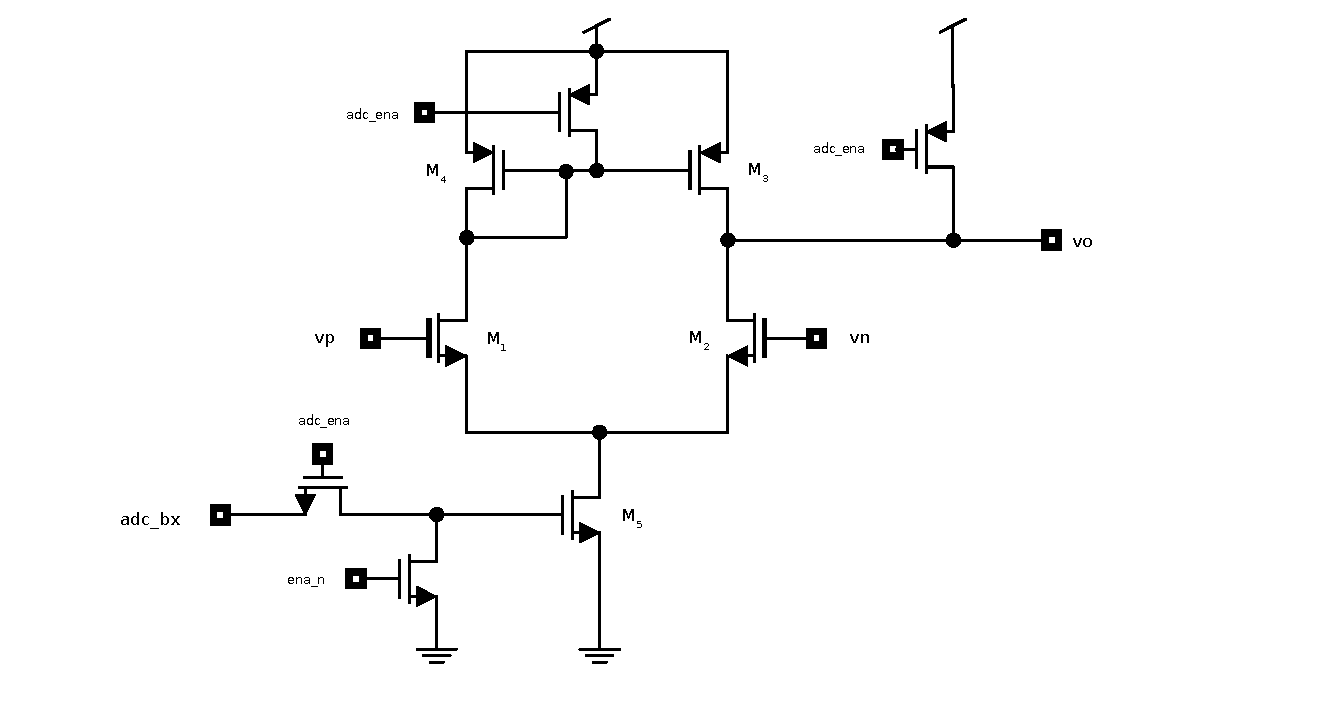
\includegraphics[width=\textwidth]{svg/ota_sch.pdf}
	\caption{Esquemático del OTA comparador}
	\label{fig:ota_sch}
\end{figure}

\paragraph{}
Los transistores $M_1$ y $M_2$ forman el par diferencial, con sus correspondiente
espejo de corrientes en $M_3$ y $M_4$, y la fuente de corriente $M_5$, el resto de
transistores sirven para deshabilitar el OTA cuando no se esté usando.

\section{Rampa analógica}\label{cap:ro_sch_armp}

\paragraph{}
El bloque generador de la rampa analógica se encuentra situado fuera del Canal de
Lectura. Se encarga de generar una señal linealmente creciente y su correspondiente
decreciente. El rango en el que la rampa varía debe ajustarse en fucnión del rango
de entrada del OTA del comparador y teniendo en cuenta el rango en el que varía
la salida del píxel, para obtener una resolución deseada y aprovechar al máximo
la sensibilidad del sensor.

\paragraph{}
Es muy importante una precisa generación de ésta rampa analógica, con especial
atención a la linealidad de la misma. En la bibliografía se describe una arquitectura
para el generador de rampa que obtiene una buena linealidad por debajo de un LSB
para resoluciones de hasta 15 bits a frecuencias de reloj de 100MHz\cite{Sordo-Ibanez2013},
que está en un rango adecuado para los tiempos de lectura que se suelen tratar en
sensores de imagen CMOS.

\paragraph{}
La señal generada debe propagarse a lo largo de lo todos los canales de lectura,
desde la izquierda hacia la derecha, o al contrario, en su caso. Para conseguir
una rápida y efectiva propagación de esta señal sin distorsión y en tiempo, ha
de hacerse un cuidadoso estudio de layout, calculando las anchuras y separaciones
entre las líneas metálicas que distribuirán la señal y posteriormente, realizando
una precisa extracción y simulación del circuito.

\paragraph{}
Por otro lado, se debe asegurar que las \textit{fases} se propaguen a una velocidad
controlada e igual al resto de señales

\section{Bloques de polarización}\label{cap:ro_sch_bias}

\paragraph{}
Los bloques del canal descritos anteriormente, la fuente de corriente y el ADC
requieren de varias señales de polarización, que habitualmente, además, suelen
ser programables, esto es, que permiten diferentes valores de configuración
establecidos por el usuario del dispositivo sobre pr ejemplo, la velocidad de
lectura, la resolución deseada, el consumo.

\paragraph{}
Normalmente, para ahorrar espacio, los bloques de polarización, o \textit{BIAS},
se comparten entre varios canales de lectura. De esta forma, el layout de estos
bloques puede ser más ancho que alto, con lo que conseguimos un ahorro de área en
la dirección vertical.

\subsection{PXCS Bias}

\paragraph{}
La fuente de corriente necesita de tres voltajes de polarización: $vb\_bn$ y
$vb\_cn$, que vienen de un espejo cascode y la tensión del limitador $vb\_ln$.
El bloque va a estar compartido por 8 canales (80$\mum$ de anchura).

\paragraph{}
Los valores de la corriente que podrá drenar la fuente de corriente del píxel, va
a ser configurable con 5 bits de resolución. Ésta configuración será implementada
en este bloque de polarización mediante 5 ramas de corrientes que conduzcan,
respectivamente, $I_0$, $2I_0$, $2I_0$, $4I_0$, $8I_0$, con
$I_0=125\nA$. De forma que podemos variar la corriente total entre $125\nA$ y
$3.875\muA$, en pasos de $125\nA$.

\subsection{ADC Bias}

\paragraph{}
El ADC Bias tiene que proveer al ADC del voltaje de modo común ($vs\_adc\_cmi$) y
de la tensión de bias de la fuente de corriente ($vb\_adc\_bx$), que espejará
una corriente generada en el Bias.

\paragraph{}
La tensión de modo común se puede generar de dos formas, la primera mediante un
buffer que replica una tensión generada en el bloque de Referencias, fuera del
canal de lectura, y la segunda generando un tensión local por cada grupo de canales.
Ésta segunda opción también usa una referencia común, pero al ser local, se adapta
mejor a la eventual curva en las alimentaciones que podremos tener a lo largo
del RO. Éste tema se tratará con más detalle en la correspondiente sección de layout.


\section{Rampa digital y serialización}

\paragraph{}
Una vez la operación de comparación se ha iniciado, la rampa y la señal del píxel,
en algún momento se cruzarán, lo que desencadenará una transición en la señal
$adc\_take$ que es la que finalmente sale de la parte analógica del canal y se va
a rutar hacia abajo para ser registrada por el contador digital.

\paragraph{}
Dicho contador (o rampa) digital habrá empezado la cuenta desde cero, en un tiempo y a una
velocidad adecuados para que el valor más alto de la cuenta digital (la resolución)
coincida con el valor final de la rampa analógica y con el valor mínimo de tensión
de salida del píxel (máxima intensidad lumínica). En el momento en que se recibe
el pulso en la salida $adc\_take$, se detiene la cuenta digital y tenemos un valor
digitalizado proporcional a la intensidad lumínica captada por el píxel actual.

\paragraph{}
El bloque que genera la rampa digital DRMP se sitúa a uno de los lados del RO y
su señal se distribuye mediante búferes digitales a lo largo del SPS, que es
el bloque digital situado debajo del Canal de Lectura y que incluye la digitalización
y serialización de los datos.

\paragraph{}
La serialización se efectúa para convertir la operación de digitalización, que se
hace de forma paralela, simulatánea a todos los canales, a una salida de datos en serie.
Éstos datos en serie se encaminan posteriormente hacia uno o varios buses de salida
del chip mediante algún protocolo de datos serie típico para poder ser almacenados
y/o procesados por otro dispositivo en el exterior del sensor de imágen.
